\section{Kacper Dłubała}
\label{sec:kdlub}

Zacznijmy od pięknego zdjęcia górskiego krajobrazu (Figure~\ref{fig:mnt}).

\begin{figure}[htbp]
    \centering
    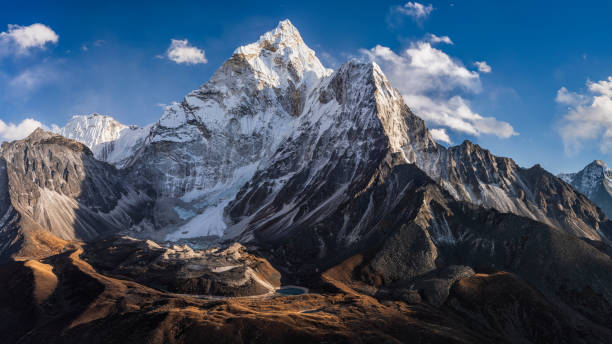
\includegraphics[width=0.5\textwidth]{pictures/gory.jpg}
    \caption{Zestaw gór.}
    \label{fig:mnt}
\end{figure}

Najlepsi speedcuberzy na świecie:
\begin{enumerate}
    \item Yiheng Wang
    \item Tymon Kolasiński
    \item Max Park
\end{enumerate}

I więcej informacji o nich (Tabela~\ref{tab:spc}) 

\begin{table}[htbp]
\begin{tabular}{|l|l|l|}
\hline
\textbf{Imię i nazwisko} & \textbf{Wynik (średnia z 5)} & \textbf{Kraj}     \\ \hline
Yiheng Wang              & 4.48                         & Chiny             \\ \hline
Tymon Kolasiński         & 4.86                         & Polska            \\ \hline
Max Park                 & 4.86                         & Stany Zjednoczone \\ \hline
\end{tabular}
\label{tab:spc}
\caption{Top 3 speedcuberów na świecie}
\end{table}

Trywialne twierdzenie\footnote{tw. Lagrange'a}: \[\exists c\in(a, b)\ : \frac{f(b)-f(a)}{b-a}=f`(c)\]
Wzór na pole trójkąta: $\frac{a*h}{2}$

\vspace{1cm}

Leonhard Euler (\textit{ur. 15 kwietnia 1707 w Bazylei, zm. 18 września 1783 w Petersburgu}) - szwajcarski \underline{matematyk i fizyk}; był pionierem w wielu obszarach obu tych nauk. Większą część życia spędził w Rosji i Prusach. Jest uważany za jednego z najbardziej płodnych matematyków w historii.

Dokonał licznych odkryć w tak różnych gałęziach matematyki jak \textbf{rachunek różniczkowy i całkowy} oraz \textbf{teoria grafów}. Wniósł duży wkład w rozwój terminologii i notacji matematycznej, szczególnie trwały w dziedzinie \textbf{analizy matematycznej}. Jako pierwszy w historii użył na przykład pojęcia \\i oznaczenia \emph{funkcji}. Opublikował wiele ważnych prac z zakresu \textbf{mechaniki}, \textbf{optyki} i \textbf{astronomii}.

\vspace{1cm}

Typy figur szachowych:
\begin{itemize}
    \item Król
    \item Hetman
    \item Wieża
    \item Goniec
    \item Skoczek
    \item Pion
\end{itemize}



